\chapter{Firmware Design}
\section{STM32CubeMX}
The robot uses an STMicroelectronics STM32F446RE microcontroller (MCU) for low level sensor interfacing and motor control signal generation. The MCU sends filtered sensor data to a Raspberry Pi \cite{raspberrypi} and receives speed and direction commands for each motor. Before starting the electrical design, the various hardware signals must be assigned to the MCU's GPIO with consideration for the device's peripherals such as timers and I\textsuperscript{2}C buses, a process aided by STMicroelectronics' configuration program, STM32CubeMX, shown in Figure \ref{fig:stm32cubemx} \cite{stm32cubemx}. Within the program, the user selects which MCU to configure and a graphical representation of the chip is shown in the GUI. The MCU's GPIO pins are arranged into banks of up to 16 pins each called ports. For example, PC2 is the second pin in Port C while PB11 is Pin 11 in Port B. The left column of the GUI lists the device peripherals including analog-to-digital converters (ADCs); various buses such as SPI, USART, and USB; and timers. Peripheral settings can be chosen here such as USART mode (asynchronous, single-wire, LIN, etc) and flow control as well as timer clock sourcing and channel modes.
\begin{figure}[H]   % [h] means here
	\centering 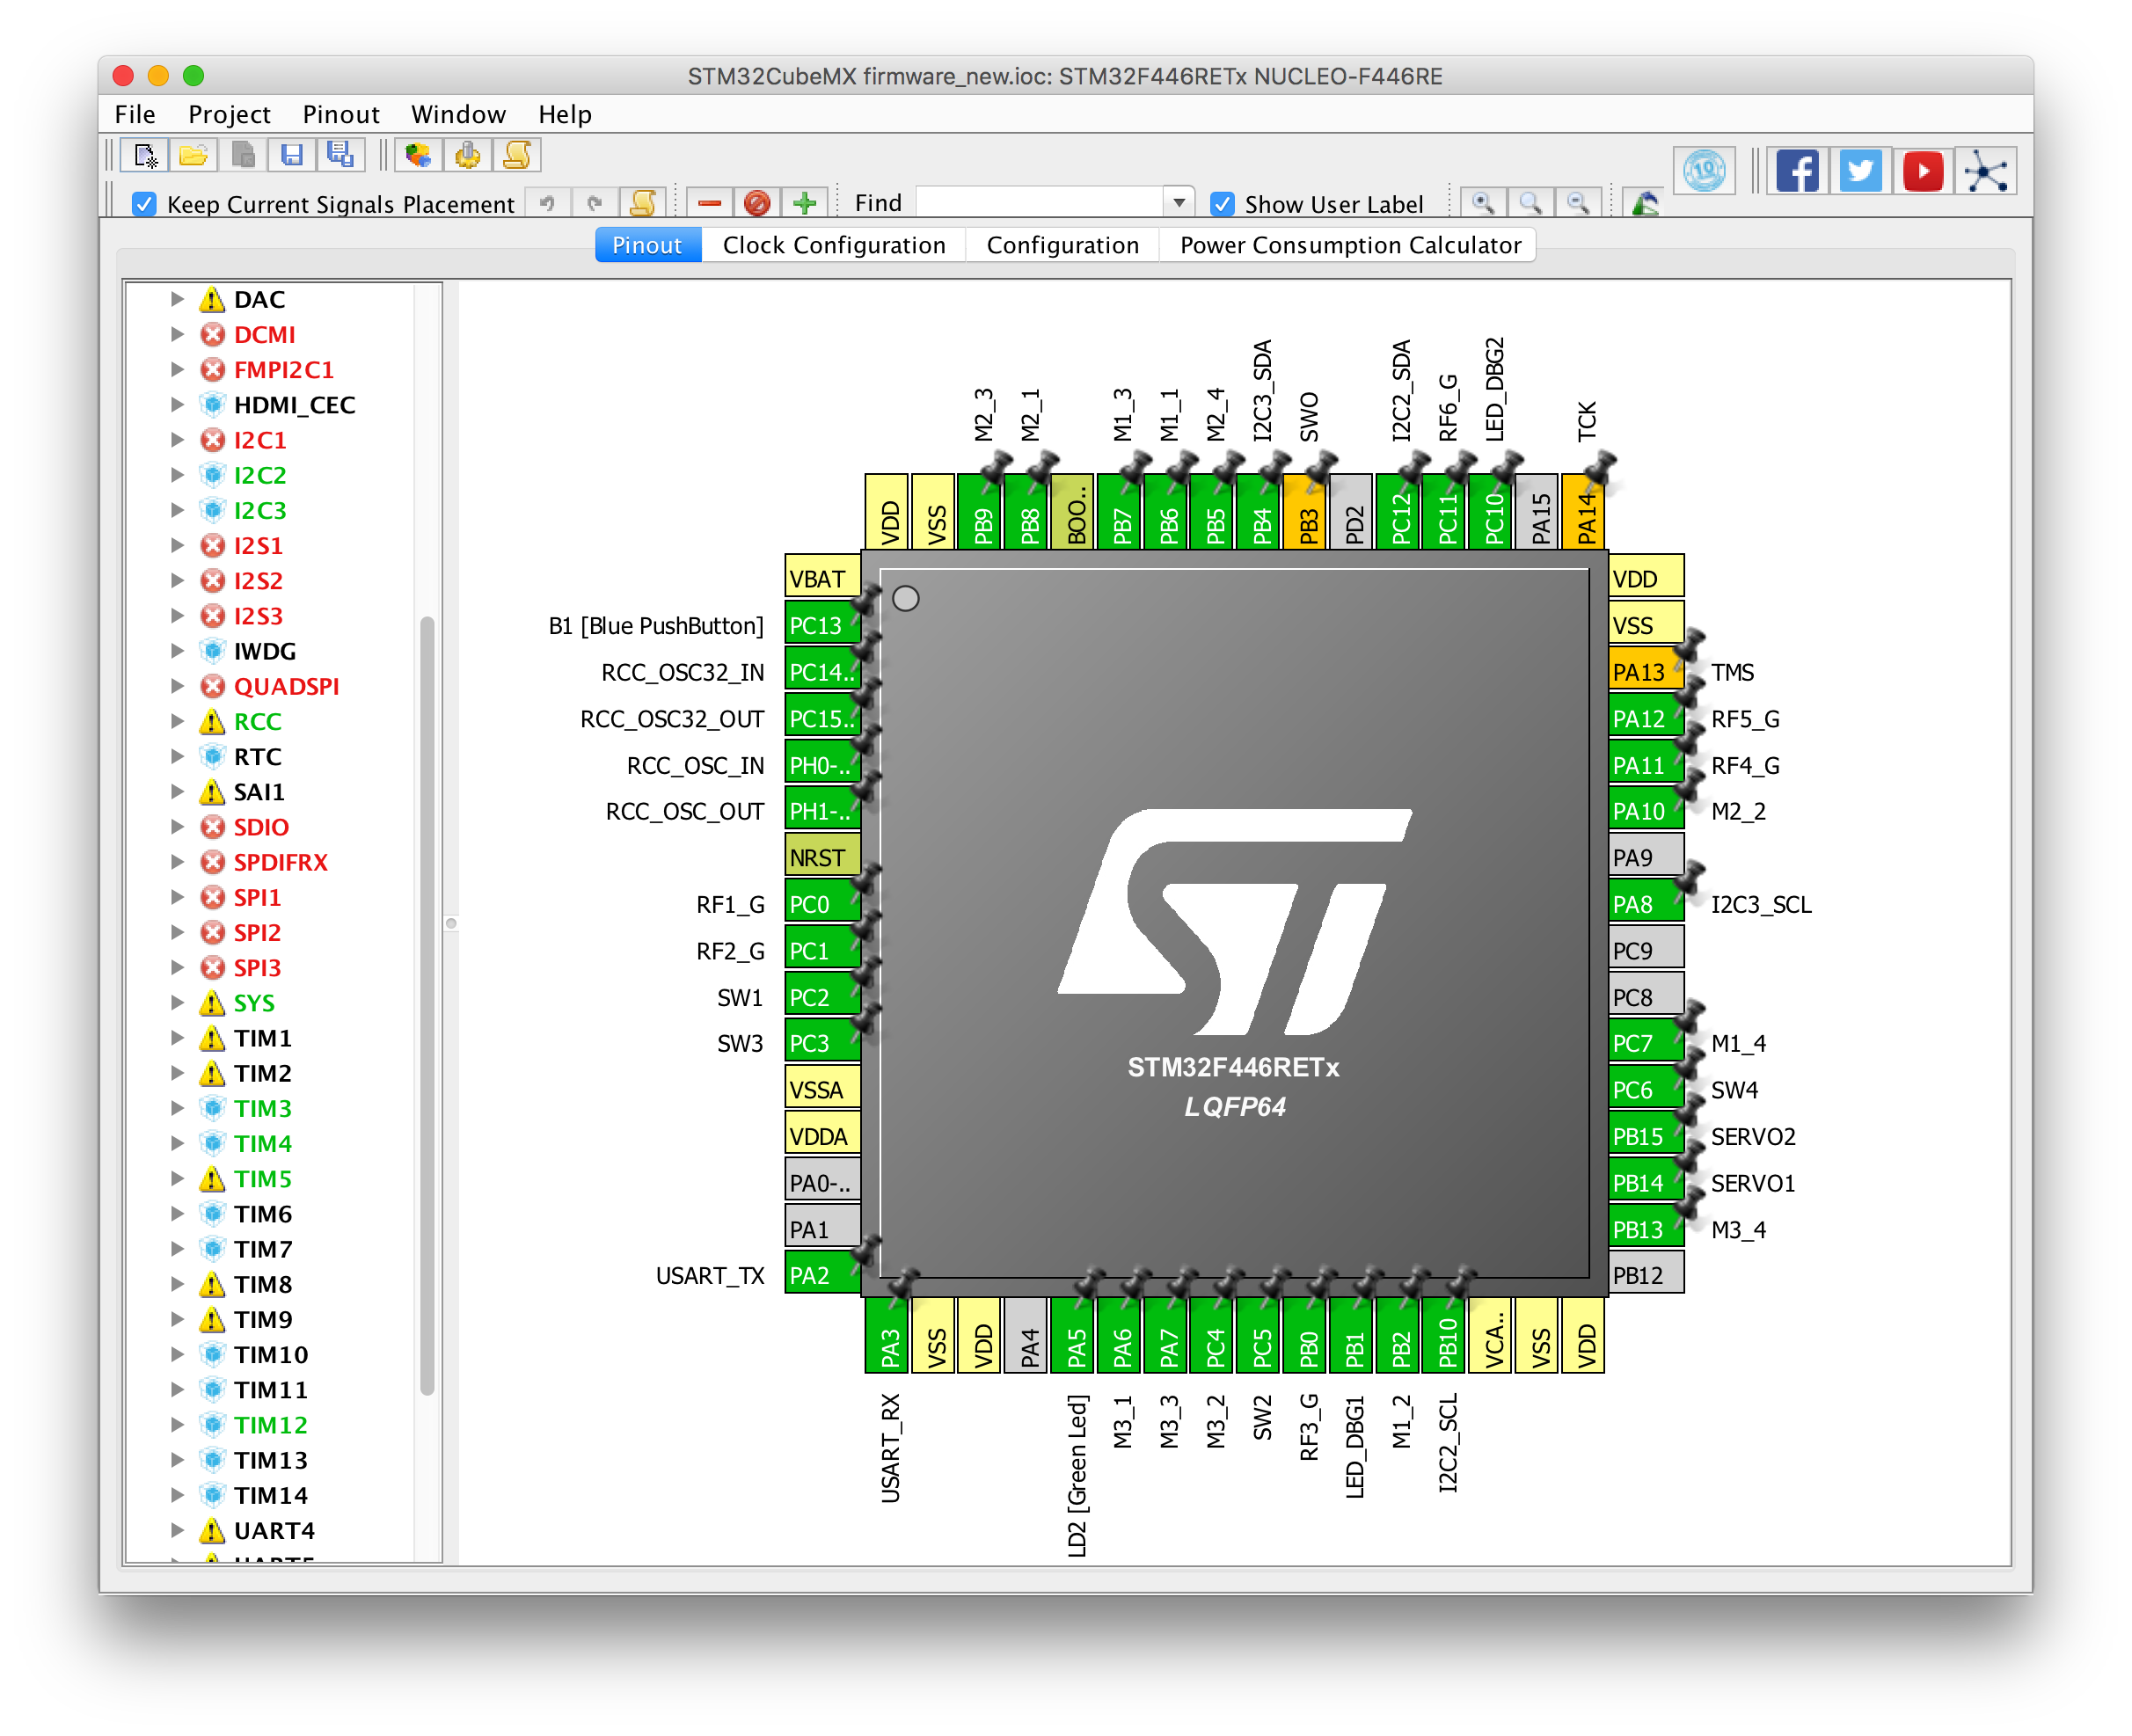
\includegraphics[width=6in, keepaspectratio]{figures/stm32cubemx.png}
	\caption{STM32CubeMX}\label{fig:stm32cubemx}
\end{figure}
The program greatly reduces development effort. Clicking a pin on the GUI brings up a menu of possible assignments. For example, clicking PB15, seen in Figure \ref{fig:stm32cubemx_pin}, shows that the pin can be used for the ADC, I2S2, as SPI2's MOSI, TIMER12's CH2 output, part of the USB differential data pair, as standard GPIO input or output, and more. As pins are assigned to various purposes, the program continually checks for compatibility issues and pin conflicts so a user can iteratively assign pins until all errors clear. For example, using a particular set of timers may actually prevent the use of I2C1 so either I2C2 or I2C3 must be used instead. This process is much faster and less error-prone than searching through the MCU's immense datasheet to manually check for assignment conflicts within every peripheral.
\begin{figure}[H]   % [h] means here
	\centering 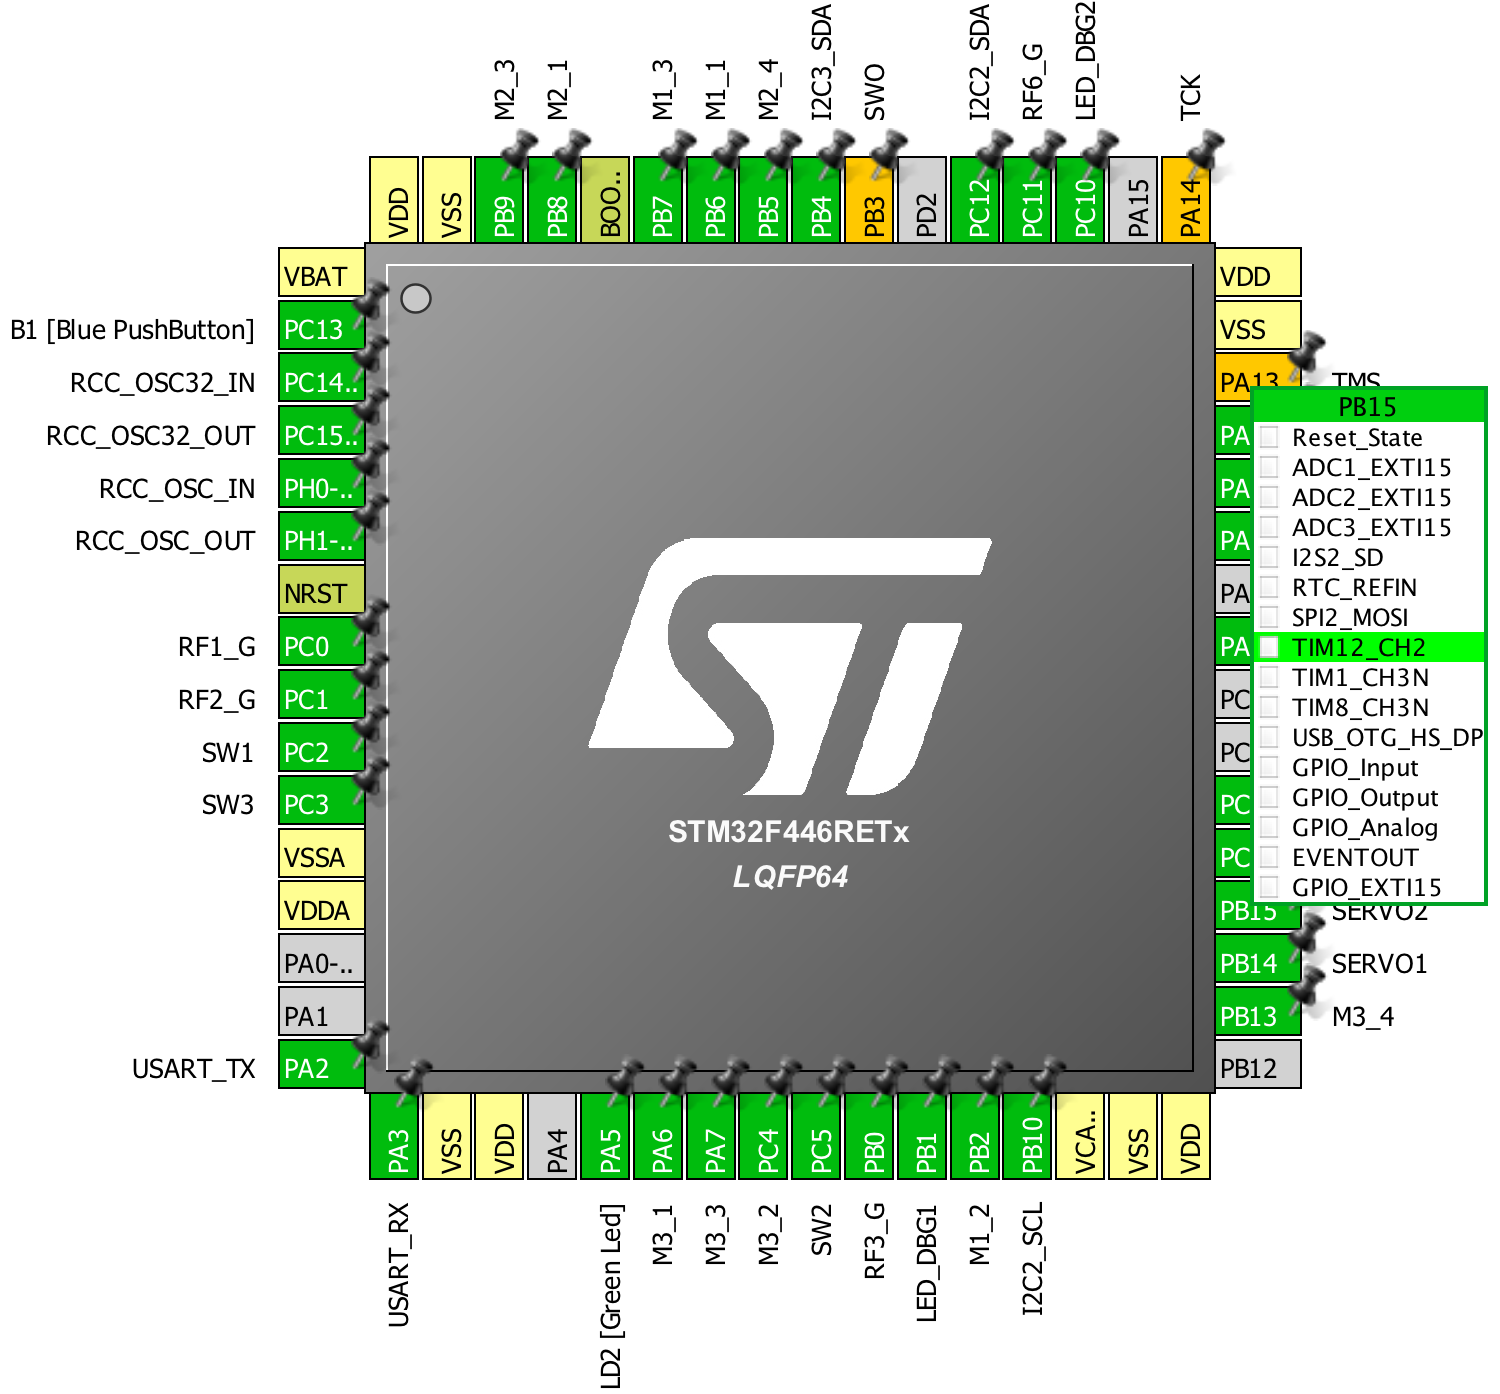
\includegraphics[width=6in, keepaspectratio]{figures/stm32cubemx_pin.png}
	\caption{STM32CubeMX -- Pin Menu}\label{fig:stm32cubemx_pin}
\end{figure}
The software also provides device-wide clock and PLL configuration as shown in Figure \ref{fig:stm32cubemx_clocks}. The MCU uses an external 8 MHz crystal to drive the internal PLL which then generates a 180 MHz system clock. Since the system is optimized for performance instead of power-saving, the advanced peripheral bus (APB) clocks run at 45 MHz and 90 MHz for APB1 and APB2, respectively \cite{stm32f446re}. 
\begin{figure}[H]   % [h] means here
	\centering 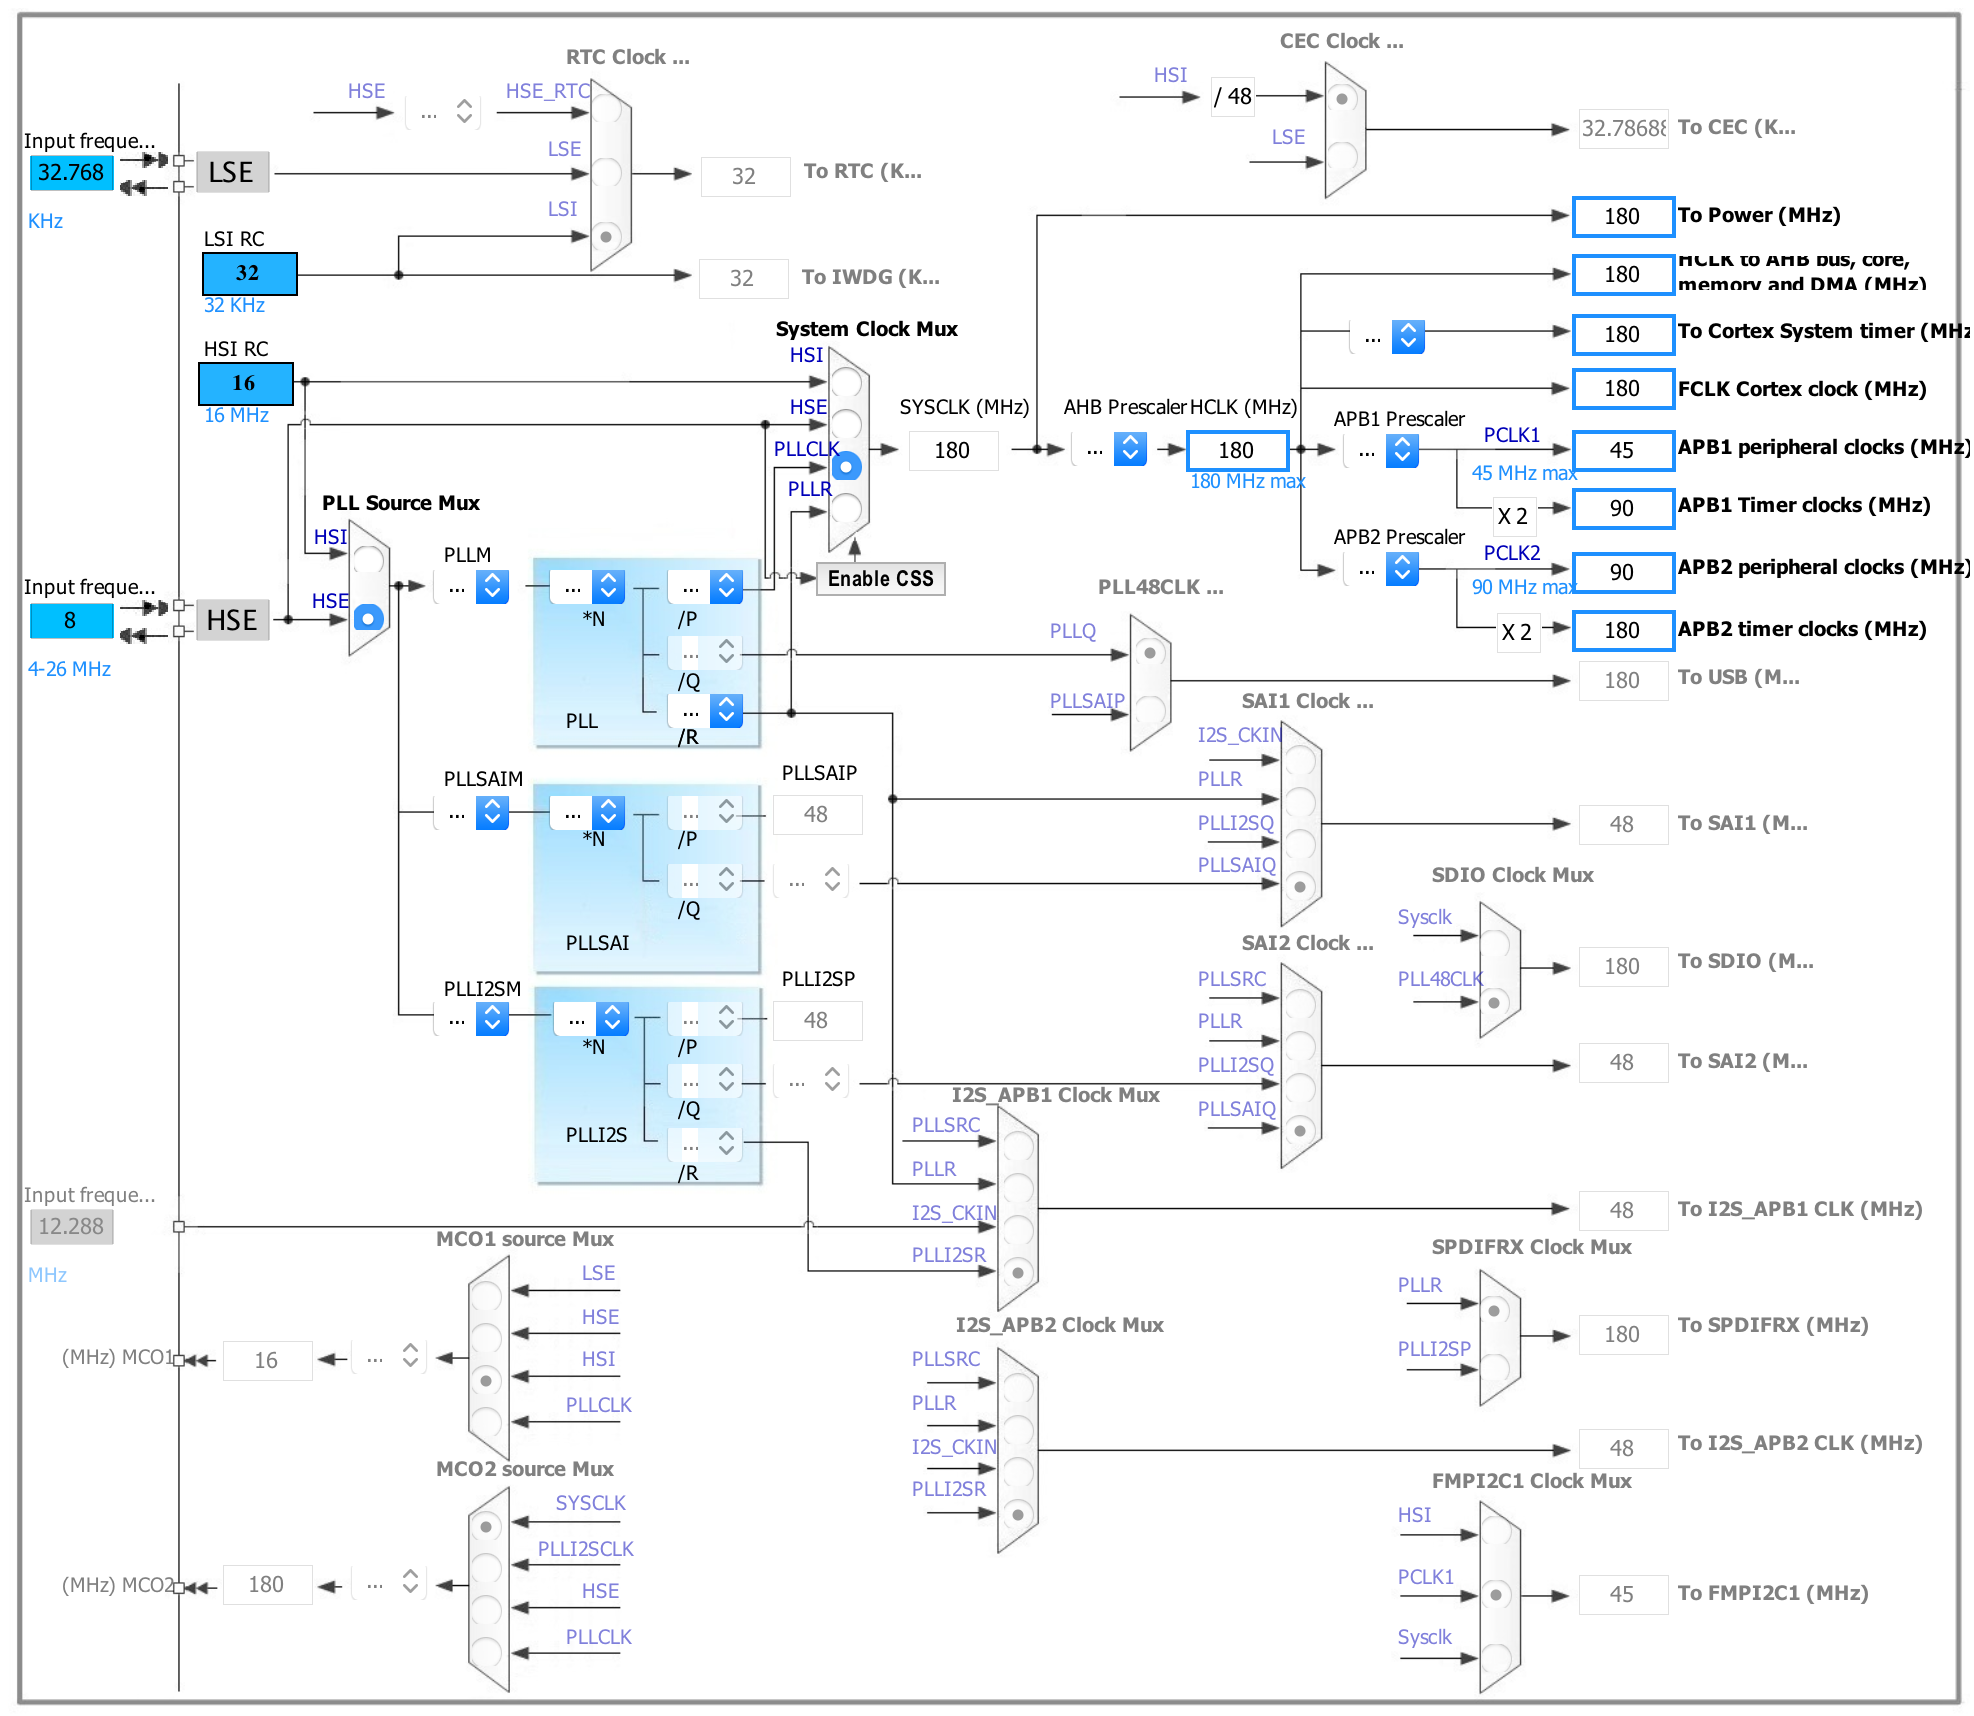
\includegraphics[width=6in, keepaspectratio]{figures/stm32cubemx_clocks.png}
	\caption{STM32CubeMX -- Clock Configurator}\label{fig:stm32cubemx_clocks}
\end{figure}
Another tab within STM32CubeMX provides detailed peripheral configuration, shown in Figure \ref{fig:stm32cubemx_config}. Both I\textsuperscript{2}C buses are set to 400 kHz with a 2:1 T\textsubscript{low}:T\textsubscript{high} duty cycle to meet the minimum pulse width requirement of slave devices. The USART peripheral is configured to 921,600 bits/s, 8-bit words, no parity, and one stop bit. The direct memory access (DMA) controller is set to process requests from the I\textsuperscript{2}C and UART peripherals to reduce processor load. 
\begin{figure}[H]   % [h] means here
	\centering 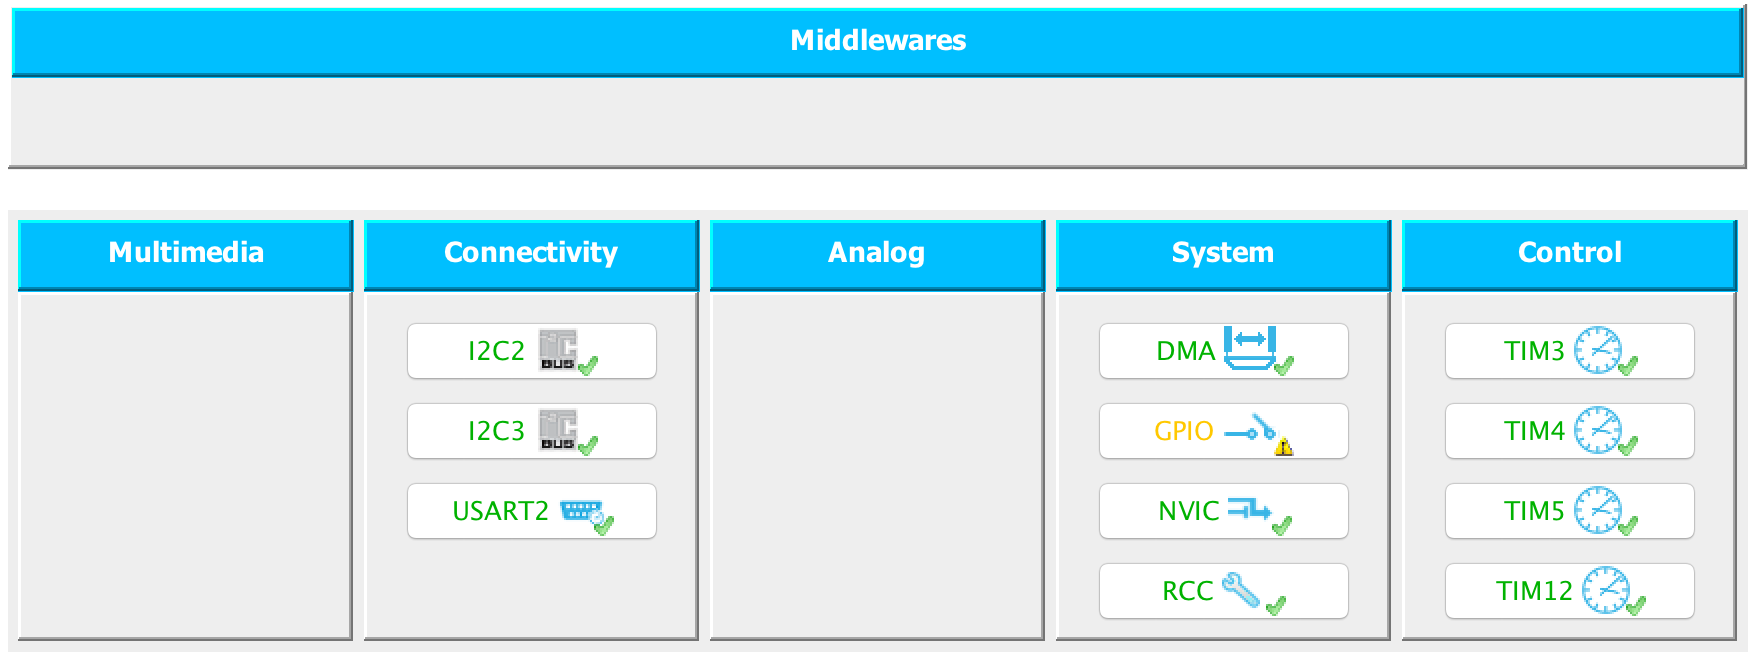
\includegraphics[width=6in, keepaspectratio]{figures/stm32cubemx_config.png}
	\caption{STM32CubeMX -- Peripheral Configurator}\label{fig:stm32cubemx_config}
\end{figure}
The robot uses four of the MCU's timers: TIMER3, TIMER4, TIMER5, and TIMER12. Each of these timers sources its base clock from the APB1 clock which is 90 MHz. TIMER3 and TIMER4 output 6 PWM control signals for the motor drivers. They are set to count upward and reset after the counter reaches 2047 to produce a 43.9 kHz PWM frequency in the ultrasonic range. TIMER5, used for delay and timing functions, employs a clock prescaler of 9000 so the counter increases every 0.1 ms and never resets; the 32-bit counter has a maximum value of 4,294,967,295 corresponding to a counter rollover period of about 5 days. Finally, TIMER12 drives the PWM signals for servo control. It uses a 45 prescaler and a 50,000 counter period to produce a 40 Hz PWM frequency.

After configuring the various items above, STM32CubeMX can generate common boilerplate plate code to initialize and configure all the devices. Include and source files are generated on a by-peripheral basis to compartmentalize code. The program also generates a report of the device configuration, attached in Appendix \ref{appendix:stm32cubemx_report}.

\section{Microcontroller Firmware}
The firmware, written in C and compiled with gcc, consists of a main file in conjunction with peripheral driver files \cite{gcc}. The dependency graph is shown in Figure \ref{fig:firmware_dependencies} with file descriptions shown in Table \ref{tab:firmware_file_desc}.  STM32CubeMX automatically generated several files to which user code was added for specific robot functions. The VL53L0X API, provided by STMicroelectronics, was also modified for the STM32F446 platform. Table \ref{tab:firmware_specs} lists the firmware requirements.
\begin{figure}[H]   % [h] means here
	\centering 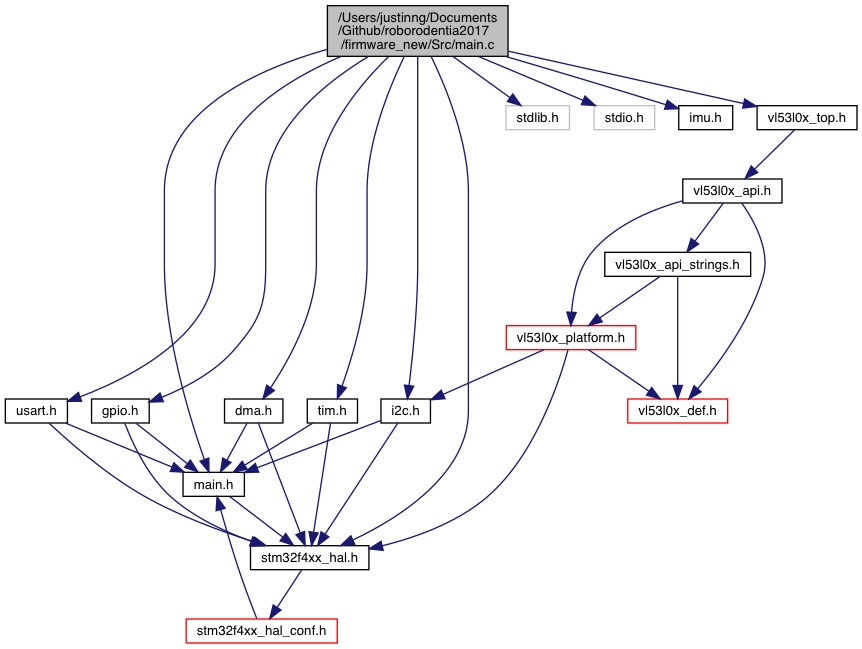
\includegraphics[width=6in,height=9in,keepaspectratio]{figures/firmware_dependencies.png}
	\caption{Firmware Dependency Graph for main.c}\label{fig:firmware_dependencies}
\end{figure}
\begin{table}[H]
	\centering	\caption{Firmware -- Source File Summary} 	\label{tab:firmware_file_desc}
	\begin{tabular}{r|l}
		\toprule 
		\multicolumn{1}{c}{File (.h/.c)} & \multicolumn{1}{c}{Description} \\ 
		\midrule 
		main & Initialization and main loop. \\  
		stm32f4xx\_hal & Hardware abstraction layer driver. \\  			
		dma & Sets up DMA priorities and enables DMA interrupts. \\  		
		i2c & Initializes I\textsuperscript{2}C buses, read/write, finds active devices. \\  		
		tim & Initializes timers 3, 4, 5, and 12. \\  		
		usart & Initializes UART, functions to write to bus, DMA callbacks. \\  		
		gpio & Configures GPIO modes (in/out), speeds, and pull-ups/pull-downs. \\  		
		vl53l0x\_top & STMicroelectronics API for configuring and reading rangefinders. \\  				 
		imu & Initializes IMU; read gyroscope, accelerometer, and magnetometer. \\ 
		\bottomrule 		
	\end{tabular} 
\end{table}
\begin{table}[H]
	\centering	\caption{Firmware -- Requirements} 	\label{tab:firmware_specs}
	\begin{tabular}{c|l}
		\toprule 
		 & \multicolumn{1}{c}{Requirements} \\ 
		 \midrule 
		1. & Initialize I\textsuperscript{2}C sensors including rangefinders and IMU. \\  
		2. & Read and store data from sensors. \\  
		3. & Filter data from sensors to reduce noise. \\  
		4. & Generate PWM signal to drive servo. \\  
		5. & Generate control signals to motor drivers. \\  
		6. & Sequence launcher motors, blower fan, and servo to fire balls. \\  
		7. & Flash LED to indicate error state. \\  
		8. & Communicate with computer over UART link. Add'l specifications in \ref{tab:firmware_uart_specs}. \\ \bottomrule 
	\end{tabular} 
\end{table}

\subsection{UART Commands}
The MCU responds to UART commands from a computer. The command syntax generally involves a sequence of one or more 8-bit characters. Table \ref{tab:firmware_uart_specs} lists the available commands. 
\begin{table}
	\centering	\caption{Firmware -- UART Commands}  \label{tab:firmware_uart_specs}
	\begin{tabularx}{\textwidth}{@{} c|Y @{}}
		\toprule 
		Syntax & \multicolumn{1}{c}{Command} \\ 
		\midrule 
		A & Start reading all rangefinders. \\  
		B & Returns sensor data in binary form (machine-readable). \\  
		D & Return sensor data in text form (human-readable). \\  
		I\textless BUS\textgreater & Scans I\textsuperscript{2}C bus and returns addresses of active devices. \\ 
		& \textless BUS\textgreater\ valid values: \\ 
		& \qquad 2 : Scan I2C2. \\
		& \qquad 3 : Scan I2C3. \\  \addlinespace
		L\textless SIDE\textgreater & Launch balls from one side of the hopper. \\
		& \textless SIDE\textgreater\ valid values: \\ 
		& \qquad L : Launch balls from left side. \\
		& \qquad R : Launch balls from right side. \\
		& \qquad S : Stop all motors. \\  \addlinespace
		M\textless FL\textgreater\textless BL\textgreater\textless BR\textgreater\textless FR\textgreater & Sets motor duty cycle calculated as \textless arg\textgreater\ divided by 2047. Each argument accepts a integer from 0 to 2047. \\
		& \textless FL\textgreater\ : PWM value for front left motor. \\
		& \textless BL\textgreater\ : PWM value for back left motor. \\
		& \textless BR\textgreater\ : PWM value for back right motor. \\
		& \textless FR\textgreater\ : PWM value for front right motor. \\  \addlinespace	
		V & Returns firmware version info. \\  
		Z & Return debug button pressed flag. \\ 
		\bottomrule 
	\end{tabularx} 
\end{table}

\subsubsection{UART Receiving}
After receiving a character on the UART bus, the DMA places it into \cinline{rxBuffer} and fires an interrupt. The MCU enters the UART receive complete DMA callback, shown in Listing \ref{list:uart_receive}, which collects the received characters into a command string stored in \cinline{stringBuffer}. If the UART receives a new line or line return character, the callback appends a null character to the string and calls \cinline{consoleCommand()} to parse and execute the command. The define \cinline{UART_RX_WRITEBACK} controls whether received characters and commands are echoed.
\begin{clisting}[caption={UART Receive Callback},label={list:uart_receive}]
#define RX_BUFFER_MAX_LENGTH 32 
#define UART_RX_WRITEBACK 0

uint8_t rxBuffer = '\000';
uint8_t stringBuffer[RX_BUFFER_MAX_LENGTH];
uint8_t stringBufferIndex;

void HAL_UART_RxCpltCallback(UART_HandleTypeDef *huart)
{
    uint8_t i;

    // Clear buffer
    if (stringBufferIndex == 0) {for (i = 0; i < RX_BUFFER_MAX_LENGTH; i++) stringBuffer[i] = 0;}	

    if ((rxBuffer != 10) && (rxBuffer != 13))	//if received data different from ascii 13 (enter)
    {
        if (stringBufferIndex < RX_BUFFER_MAX_LENGTH){
            stringBuffer[stringBufferIndex++] = rxBuffer; //add data to stringBuffer
        }
    }
    else // If received data = 10 or 13
    {
        if (stringBufferIndex < RX_BUFFER_MAX_LENGTH){
            stringBuffer[stringBufferIndex++] = '\0'; //add null char
        } else {
            stringBuffer[RX_BUFFER_MAX_LENGTH] = '\0'; //add null char
        }

        if (UART_RX_WRITEBACK){
            HAL_UART_Transmit(&huart2, (uint8_t *)&stringBuffer, stringBufferIndex, 0xFFFF);
            printf("\r\n");
        }
        consoleCommand((uint8_t *)&stringBuffer, stringBufferIndex);
        stringBufferIndex = 0;
    }

    if (UART_RX_WRITEBACK){
        HAL_UART_Transmit(&huart2, (uint8_t *)&rxBuffer, 1, 1);
    }
}
\end{clisting}

\subsubsection{UART Transmitting}
The \cinline{\_write()} function is overridden to redirect \cinline{printf()} output to UART using the code in Listing \ref{list:redirect_printf}.
\begin{clisting}[caption={Redirect printf()},label={list:redirect_printf}]
// Redirect printf to UART
int _write (int fd, char *ptr, int len) 
{ 
	transmitUART(ptr, len);
	return len; 
}
\end{clisting}

To avoid spending CPU cycles waiting for UART transmission to complete, the DMA buffers the character array directly to the peripheral. A flag, \cinline{txInProg}, prevents subsequent transmission until the UART transmit DMA callback, \cinline{HAL_UART_TxCpltCallback()}, clears the flag when the current transmission completes.
\begin{clisting}[caption={UART Transmit},label={list:uart_transmit}]
#define TX_BUFFER_MAX_LENGTH 2000 

uint8_t txBuffer[TX_BUFFER_MAX_LENGTH];
volatile uint8_t txInProg = 0;

// Transmit characters over UART
void transmitUART(char *ptr, int len)
{  
    // Check that the input isn't longer than our buffer
    if (len > TX_BUFFER_MAX_LENGTH){
        _Error_Handler(__FILE__, __LINE__);
    }
    // Wait until UART TX is finished
    while(txInProg == 1){}
    txInProg = 1;
    // Transfer the data to be sent into the txBuffer
    memcpy(txBuffer,(uint8_t *)ptr,len);
    HAL_UART_Transmit_DMA(&huart2, txBuffer, len); 
}

void HAL_UART_TxCpltCallback(UART_HandleTypeDef *huart)
{
    // Clear TX in progress flag when complete with transfer
    txInProg= 0;
}
\end{clisting}

\subsection{MCU Execution Flow}
The execution flow is as follows:
\begin{enumerate}
	\item Define and initialize a struct for motor pins and timer channels.
	\begin{clisting}[caption={Motor Struct},label={list:motor_struct}]
struct motor_t {
    GPIO_TypeDef *GPIOx;
    uint16_t GPIO_Pin;
    GPIO_PinState PinState;

    TIM_HandleTypeDef *TIM_Handle;
    TIM_OC_InitTypeDef sConfigOC;
    uint32_t TIM_Channel;
};

struct motor_t motorConfigs[4] = { 
    {MOTOR_FL_DIR_GPIO_Port, MOTOR_FL_DIR_Pin, GPIO_PIN_RESET, 0, {0}, TIM_CHANNEL_2}, 
    {MOTOR_FR_DIR_GPIO_Port, MOTOR_FR_DIR_Pin, GPIO_PIN_RESET, 0, {0}, TIM_CHANNEL_4}, 
    {MOTOR_BR_DIR_GPIO_Port, MOTOR_BR_DIR_Pin, GPIO_PIN_RESET, 0, {0}, TIM_CHANNEL_1}, 
    {MOTOR_BL_DIR_GPIO_Port, MOTOR_BL_DIR_Pin, GPIO_PIN_RESET, 0, {0}, TIM_CHANNEL_3}}; 
struct motor_t* motorConfigsPtr = motorConfigs;
	\end{clisting}
	\item Instantiate some variables.
	\begin{clisting}[caption={Communications Variables Initialization},label={list:comms_var_init}]
unsigned char data_packet[21];				// Holds sensor data for UART transmission
volatile uint8_t wd_reset = 0;				// Watchdog reset flag
volatile uint8_t sensor_update_req = 0;		// Queue rangefinder read flag
volatile uint8_t dbg_btn_latch = 0;			// Debug button latch
	\end{clisting}
	\item Enable all clocks since power saving not necessary.
	\begin{clisting}[caption={Enabling Clocks},label={list:enable_clocks}]
RCC->AHB1ENR |= 0xFFFFFFFF;
RCC->AHB2ENR |= 0xFFFFFFFF;
RCC->AHB3ENR |= 0xFFFFFFFF;
RCC->APB1ENR |= 0xFFFFFFFF;
RCC->APB2ENR |= 0xFFFFFFFF;
	\end{clisting}
	\item Reset peripherals, initialize SysTick, set up PLL and clocks.
	\begin{clisting}[caption={HAL and System Clock Initialization},label={list:hal_sysclk_init}]
HAL_Init();
SystemClock_Config();
	\end{clisting}
	\item Initialize configured peripherals.
	\begin{clisting}[caption={Peripheral Initialization},label={list:periph_init}]
MX_GPIO_Init();
MX_DMA_Init();
MX_I2C2_Init();
MX_I2C3_Init();
MX_TIM3_Init();
MX_TIM4_Init();
MX_TIM12_Init();
MX_USART2_UART_Init();
MX_TIM5_Init();
	\end{clisting}
	\item Reset system timer, enable UART receive DMA, initialize sensors.
	\begin{clisting}[caption={UART Service and Sensor Initialization},label={list:uart_sensor_init}]
TimeStamp_Reset();
serviceUART();
printf("Enabling IMU...\r\n");
IMU_begin();
printf("Initializing rangefinders...\r\n");
VL53L0X_begin();
	\end{clisting}
	\item Set servo to starting position.
	\begin{clisting}[caption={Servo Default Position},label={list:servo_default}]
if (HAL_TIM_PWM_Start(&htim12, TIM_CHANNEL_1) != HAL_OK){ Error_Handler(); }
	\end{clisting}
	\item Initialize variables and begin main loop.
	\begin{clisting}[caption={Loop Variables and Start},label={list:loop_start}]
uint32_t wd_start = 0;		// Watchdog start time
uint32_t cur_time = 0;		// Current time
uint8_t wd_en = 0;			// Watchdog enable
data_packet[20] = '\n';		// 21 byte sensor data packet to send over UART

while (1)
{
	\end{clisting}
	\item Watchdog prevents motors from running when UART is inactive. Receiving any UART command sets \cinline{wd\_reset} to 1.
	\begin{clisting}[caption={Motor Watchdog},label={list:motor_watchdog}]
	// Reset watchdog start time if flag is set
	if (wd_reset == 1){
		wd_start = TimeStamp_Get();  // Units of 0.1 ms based on Timer5
		wd_en = 1;
		wd_reset = 0;
	} else if (wd_en == 1){
		// Trigger if watchdog is enabled and expires
		cur_time = TimeStamp_Get();
		if ((cur_time - wd_start) > WD_LEN){
			wd_en = 0;
			
			// Disable motors
			int i;
			for (i=0; i<4; i++) {
				motorConfigs[i].PinState = GPIO_PIN_RESET;
				motorConfigs[i].sConfigOC.Pulse = 0; 
			}
			for (i=0; i<4; i++) {
				// Alter the PWM duty cycle and start PWM again
				if (HAL_TIM_PWM_ConfigChannel(motorConfigs[i].TIM_Handle, &motorConfigs[i].sConfigOC,
					motorConfigs[i].TIM_Channel) != HAL_OK) { Error_Handler(); }
				if (HAL_TIM_PWM_Start(motorConfigs[i].TIM_Handle, motorConfigs[i].TIM_Channel)
					!= HAL_OK){ Error_Handler(); }
				
				// Set the direction pin
				HAL_GPIO_WritePin(motorConfigs[i].GPIOx, motorConfigs[i].GPIO_Pin, motorConfigs[i].PinState);
			}
		}
	}											
	\end{clisting}
	\item Read debug tactile button state and latch it until read by UART.
	\begin{clisting}[caption={Debug Button Latch},label={list:dbg_btn_latch}]
	// Read debug button
	dbg_btn_latch = HAL_GPIO_ReadPin(B1_GPIO_Port, B1_Pin) && dbg_btn_latch;
	\end{clisting}
	\item If requested over UART, read all four rangefinders and store the data in the \cinline{data\_packet}.
	\begin{clisting}[caption={Rangefinder Read},label={list:range_read}]
	if (sensor_update_req == 1){
		int i;
		for (i = 0; i < 4; i++){
			if (rangefinderRead(i)){
				data_packet[i*2  ] = (rangeData[i] >> 8) & 0xFF;
				data_packet[i*2+1] =  rangeData[i]       & 0xFF;
			}
		}
		sensor_update_req = 0;
	}	
	\end{clisting}
	\item Read the magnetometer and store the data in the data packet.
	\begin{clisting}[caption={Magnetometer Read},label={list:mag_read}]
	magnetometer_read();
	data_packet[ 8] = (magData.x >> 8) & 0xFF;
	data_packet[ 9] =  magData.x       & 0xFF;
	data_packet[10] = (magData.y >> 8) & 0xFF;
	data_packet[11] =  magData.y       & 0xFF;
	data_packet[12] = (magData.z >> 8) & 0xFF;
	data_packet[13] =  magData.z       & 0xFF;	
	\end{clisting}
	\item Read the accelerometer and store the data in the data packet.
	\begin{clisting}[caption={Accelerometer Read},label={list:acc_read}]
	accelerometer_read();
	data_packet[14] = (accelData.x >> 8) & 0xFF;
	data_packet[15] =  accelData.x       & 0xFF;
	data_packet[16] = (accelData.y >> 8) & 0xFF;
	data_packet[17] =  accelData.y       & 0xFF;
	data_packet[18] = (accelData.z >> 8) & 0xFF;
	data_packet[19] =  accelData.z       & 0xFF;
}	
	\end{clisting}		
	\item Return to start of loop.
\end{enumerate}

\subsection{Error Handler}
During errors or faults, the MCU enters the error handler, prints an error message, and flashes the debug LED at 5 Hz.
\begin{clisting}[caption={Error Handler},label={list:error_handler}]
void _Error_Handler(char * file, int line)
{
	printf("Entered error handler.\r\n");
	while(1) 
	{
		HAL_GPIO_TogglePin(GPIOB, GPIO_PIN_1);
		HAL_Delay(100);
	}
}
\end{clisting}
